\documentclass[tikz,border=2pt]{standalone}
\usepackage{amsmath,amssymb}
\usepackage{pgfplots}
\pgfplotsset{compat=1.18}
\usetikzlibrary{arrows.meta}

\begin{document}
% a_n = sin(n)/n (blue): the terms get arbitrarily close to each other (Cauchy).
% b_n = sin n (red): terms keep jumping between about -1 and 1 (not Cauchy).
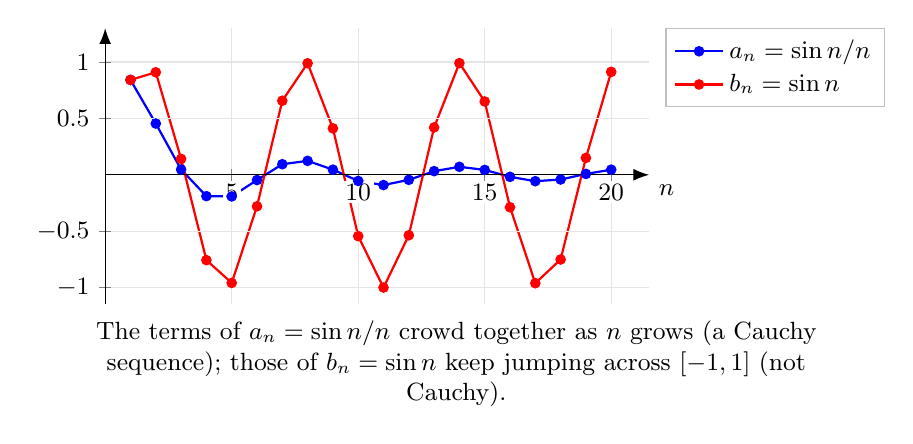
\begin{tikzpicture}[every node/.style={font=\small}]
	\begin{axis}[
		width=8.49cm, height=5.09cm,
		axis lines=middle, axis line style={-{Latex[length=2mm]}},
		xmin=0, xmax=21.5, ymin=-1.15, ymax=1.3,
		xtick={5,10,15,20}, ytick={-1,-0.5,0.5,1}, xticklabel style={fill=white, inner sep=1pt}, axis on top,
		tick label style={font=\small},
		xlabel={$n$}, xlabel style={below right},
		grid=major, grid style={gray!20},
		legend pos=outer north east, legend cell align={left},
		legend style={font=\small, draw=gray!50, fill=white},
		clip=false
		]
		\addplot[blue, thick, mark=*, mark size=1.5pt, samples at={1,...,20}] {sin(deg(x))/x};
		\addlegendentry{$a_n=\sin n/n$}
		\addplot[red, thick, mark=*, mark size=1.5pt, samples at={1,...,20}] {sin(deg(x))};
		\addlegendentry{$b_n=\sin n$}
	\end{axis}
	\node[anchor=north, align=flush center, text width=9.6cm] at ([yshift=-2pt]current bounding box.south) {The terms of $a_n=\sin n/n$ crowd together as $n$ grows (a Cauchy sequence); those of $b_n=\sin n$ keep jumping across $[-1,1]$ (not Cauchy).};
\end{tikzpicture}
\end{document}
